\subsubsection{Risultati sperimentali}

% TODO: describe simulation results
\autoref{fig:obj3_boxplot_population} mostra la distribuzione della Popolazione media al variare del rate di arrivi esterni. È possibile notare come i valori esplodano al superamento di $\lambda = 1.2 req/s$, valore oltre il quale il sistema risulta instabile. Ciò provoca anche un'esplosione dei tempi di risposta, visibile in \autoref{fig:obj3_boxplot_rtime}.

\autoref{fig:obj3_boxplot_throughput} mostra come il Throughput globale medio non vada oltre un upper bound posto tra $1.2$ e $1.4 req/s$, ulteriore conferma del fatto che il sistema non riesca a gestire efficacemente uno scenario di carico cosi pesante.

\autoref{fig:obj3_boxplot_utilization} mostra che di fatti è il server B a soffrire di più il carico poiché la sua utilizzazione diventa fissa a 1 per tassi di arrivo oltre $1.2 req/s$. Il suo throughput è anche tra i più bassi tra i server, come è visibile in \autoref{fig:obj3_lineplot_throughput_comparison}. 

\begin{figure*}
    \centering
    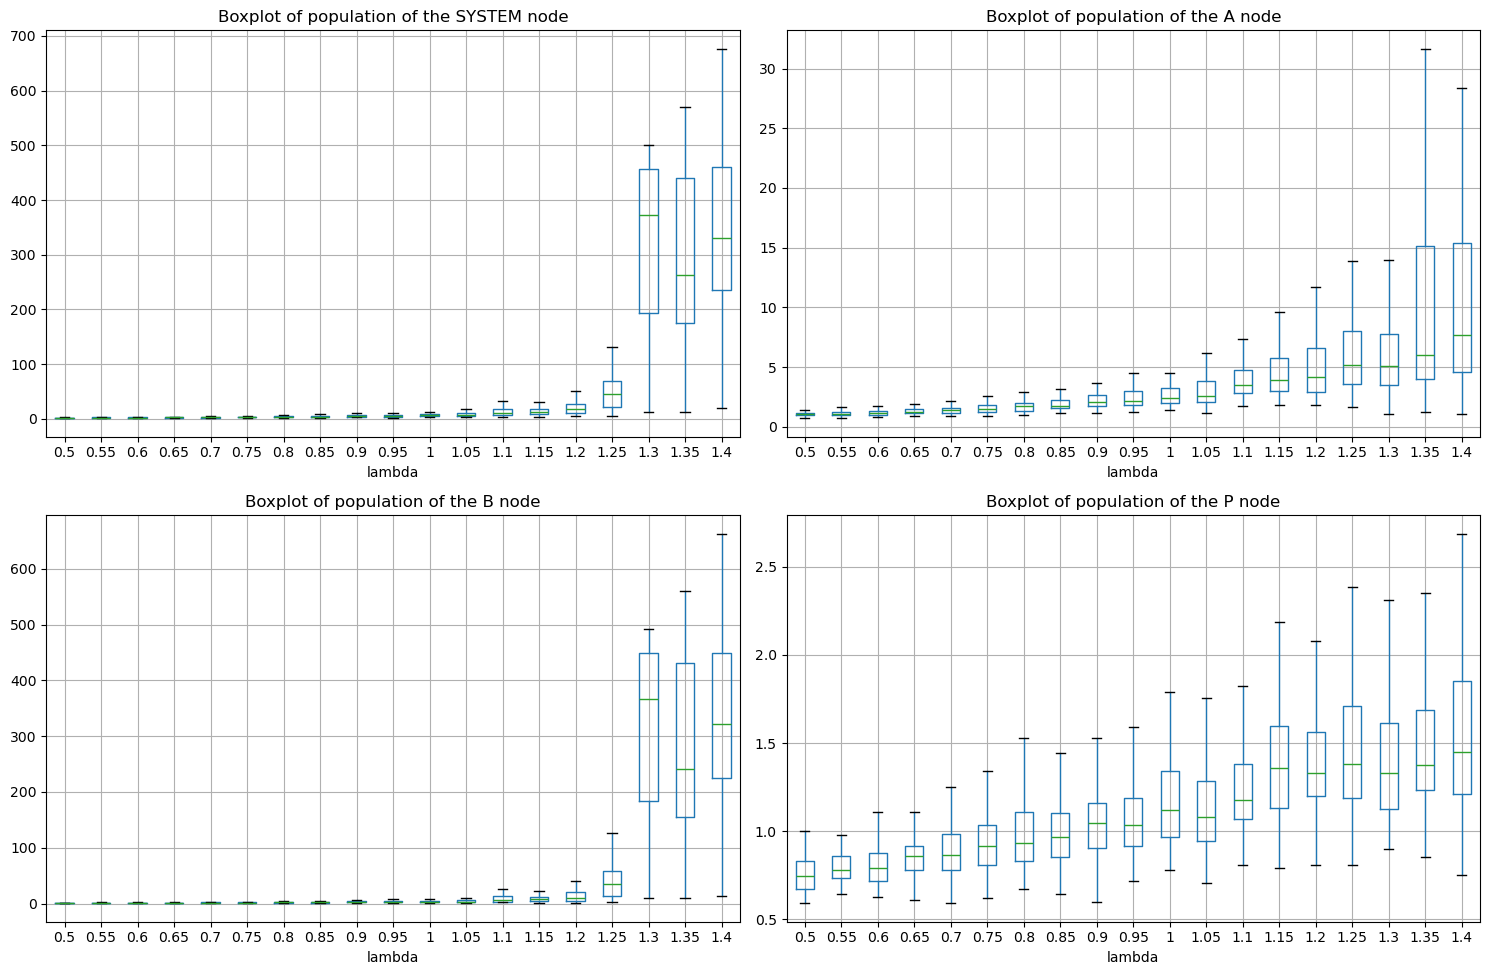
\includegraphics[width=1\linewidth]{figs//results//obj3//simulation/obj3_boxplots_population.png}
    \caption{Distribuzione della Popolazione media dei risultati sperimentali dell'obbiettivo 3.}
    \label{fig:obj3_boxplot_population}
\end{figure*}

\begin{figure*}
    \centering
    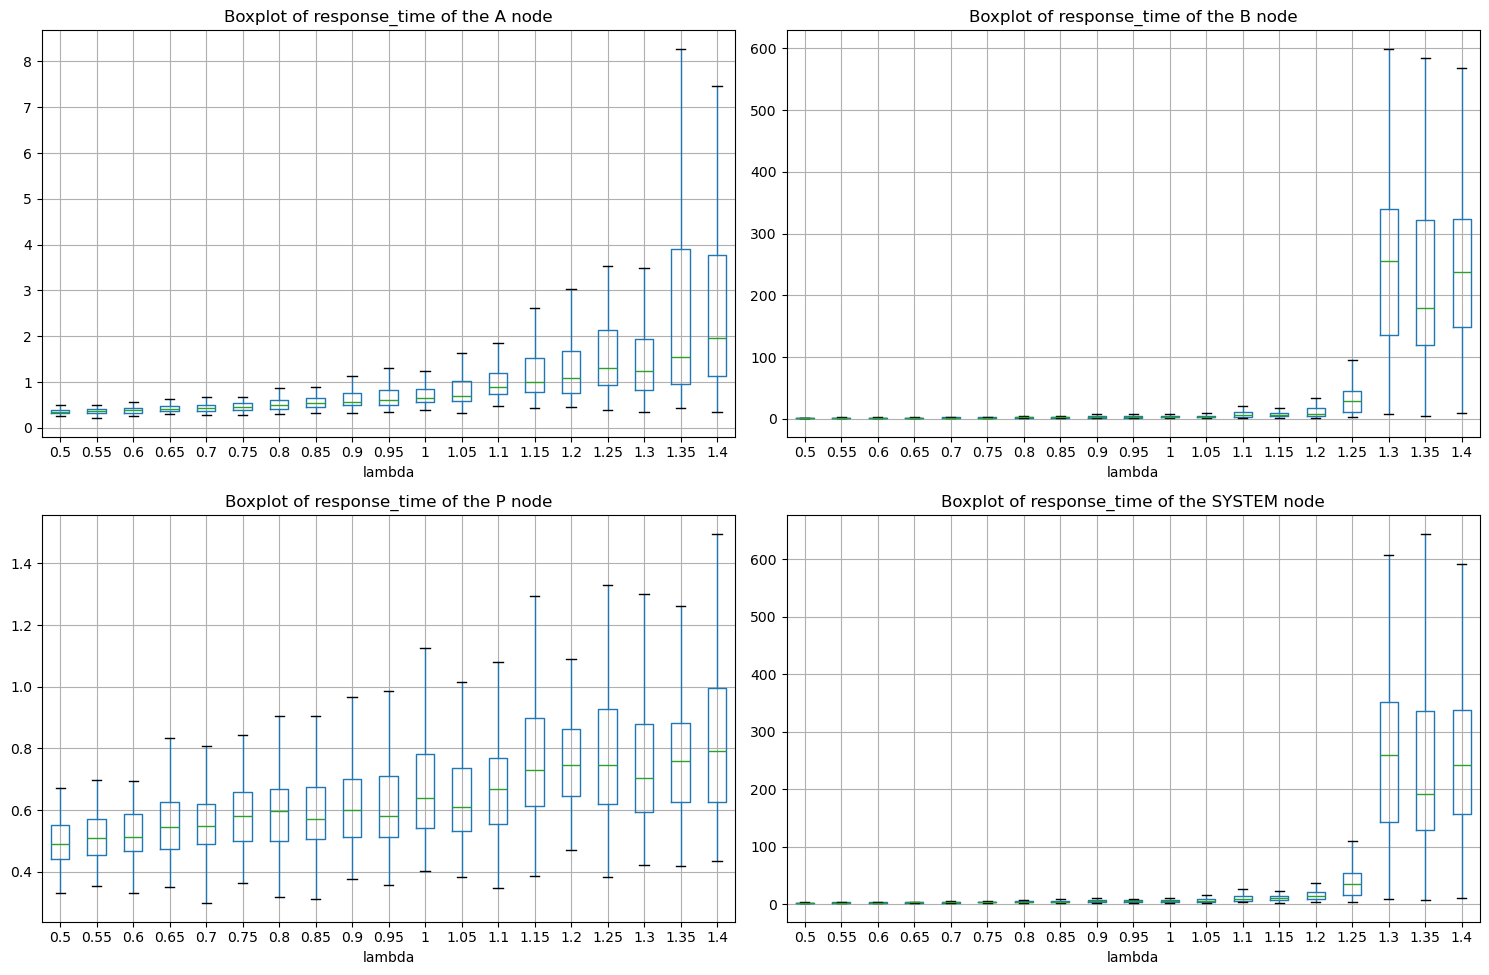
\includegraphics[width=1\linewidth]{figs//results//obj3//simulation/obj3_boxplot_rtime.png}
    \caption{Distribuzione del Tempo di Risposta medio dei risultati sperimentali dell'obbiettivo 3.}
    \label{fig:obj3_boxplot_rtime}
\end{figure*}

\begin{figure*}
    \centering
    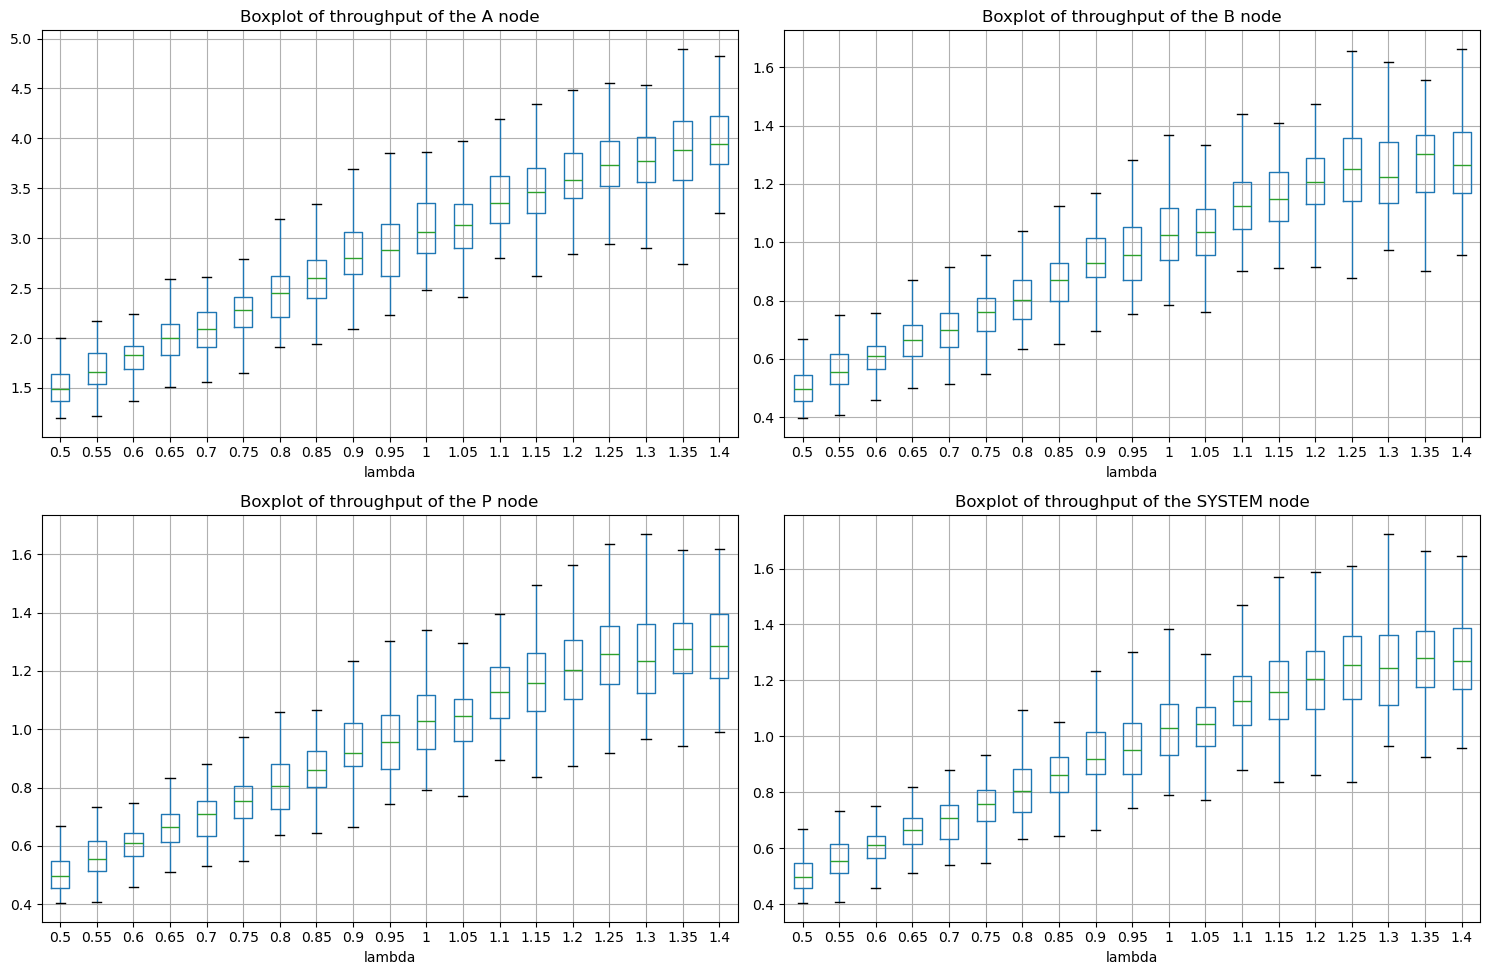
\includegraphics[width=1\linewidth]{figs//results//obj3//simulation/obj3_boxplot_throughput.png}
    \caption{Distribuzione del Throughput medio dei risultati sperimentali dell'obbiettivo 3.}
    \label{fig:obj3_boxplot_throughput}
\end{figure*}

\begin{figure*}
    \centering
    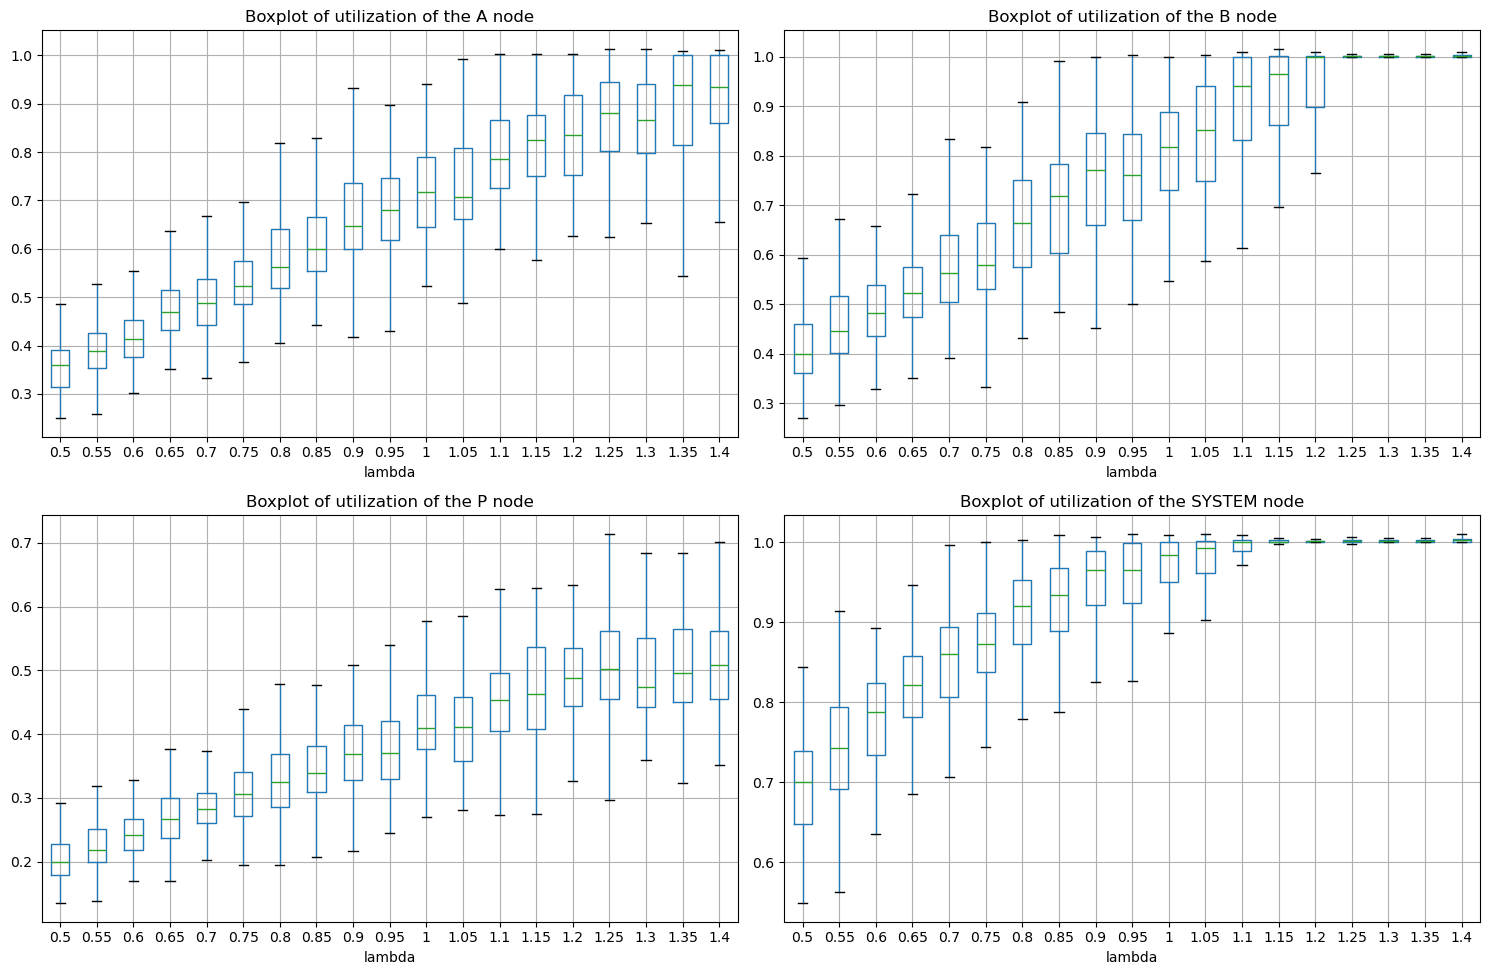
\includegraphics[width=1\linewidth]{figs//results//obj3//simulation/obj3_boxplot_utilization.png}
    \caption{Distribuzione dell'utilizzazione media dei risultati sperimentali dell'obbiettivo 3.}
    \label{fig:obj3_boxplot_utilization}
\end{figure*}

\begin{figure}[H]
    \centering
    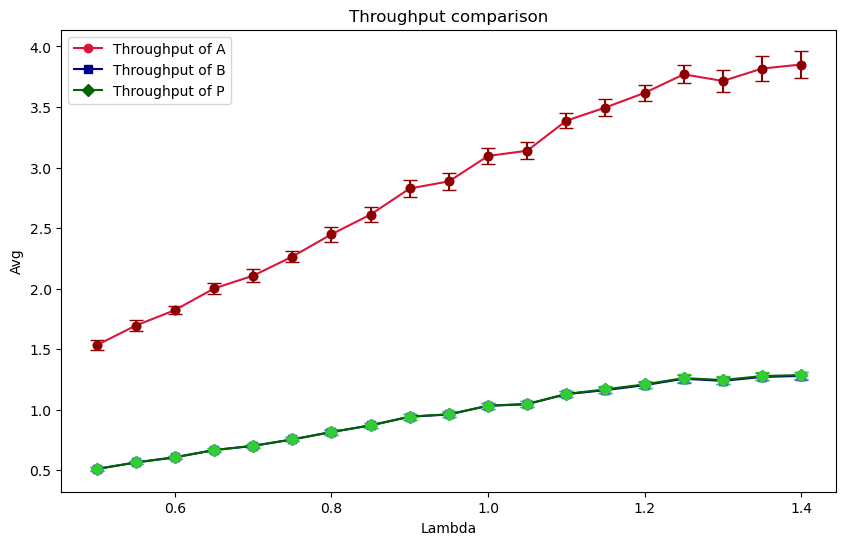
\includegraphics[width=1\linewidth]{figs//results//obj3//simulation/obj3_lineplot_throughput_comparison.png}
    \caption{Confronto dei Throughput medi tra i Server della Web App per l'obbiettivo 3. }
    \label{fig:obj3_lineplot_throughput_comparison}
\end{figure}

\subsubsection{Verifica con il modello analitico}

Il modello analitico è analogo a quanto riportato in \autoref{sec:results_obj2_verication} fino a $\lambda = 1.2 req/s$, oltre il quale non si hanno a disposizione dati analitici poiché il modello assume un regime di stazionarietà.

% \textbf{Modello analitico utilizzazione}\\
\begin{table}[!htbp]
    \centering
    \begin{tabular}{cccc}
        $\gamma$ & $\rho_{A}$ & $\rho_{B}$ & $\rho_{P}$ \\         
        0.5 & 0.257 & 0.4 & 0.2 \\
        1.4 & 0.72 & 1.12 & 0.56 \\
    \end{tabular}
    \label{tab:rho_values_last}
\end{table}

\textbf{Modello analitico indici locali}\\

\begin{table}[!htbp]
    \centering
    \begin{tabular}{cccc}
        $\gamma$ & $E[T]_{A}$ & $E[T]_{B}$ & $E[T]_{P}$ \\         
        0.5 & 0.230 & 1.333 & 0.5 \\
        1.2 & 0.447 & 20 & 0.769 \\
    \end{tabular}
    \label{tab:et_values_new}
\end{table}
\begin{table}[!htbp]
    \centering
    \begin{tabular}{cccc}
        $\gamma$ & $E[N]_{A}$ & $E[N]_{B}$ & $E[N]_{P}$ \\         
        0.5 & 0.346 & 0.666 & 0.25 \\
        1.2 & 1.611 & 24 & 0.923 \\
    \end{tabular}
    \label{tab:en_values_new}
\end{table}
\begin{table}[!htbp]
    \centering
    \begin{tabular}{cccc}
        $\gamma$ & $X_{A}$ & $X_{B}$ & $X_{P}$ \\         
        0.5 & 1.5 & 0.5 & 0.5 \\
        1.2 & 3.6 & 1.2 & 1.2 \\
    \end{tabular}
    \label{tab:x_values_new}
\end{table}

\textbf{Modello analitico indici globali}\\

\begin{table}[!htbp]
    \centering
    \begin{tabular}{cccc}
        $\gamma$ & $E[T]_{S}$ & $E[N]_{S}$ & $X_{S}$ \\         
        0.5 & 2.525 & 1.262 & 0.5 \\
        1.2 & 22.112 & 26.535 & 1.2 \\
    \end{tabular}
    \label{tab:et_en_x_values}
\end{table}

\subsubsection{Validazione con il caso di studio}
Per la validazione dei risultati si faccia riferimento a \autoref{sec:results-obj4-validation}.
